% Replace the existing fig:roadmap environment AND its next three explanatory paragraphs.
% Compile from workshop_v2/论文/. Keep exactly one fig:roadmap label.
% A4 paper: target about 160 mm text width; setting width alone preserves the aspect ratio.
\begin{figure}[htbp]\centering
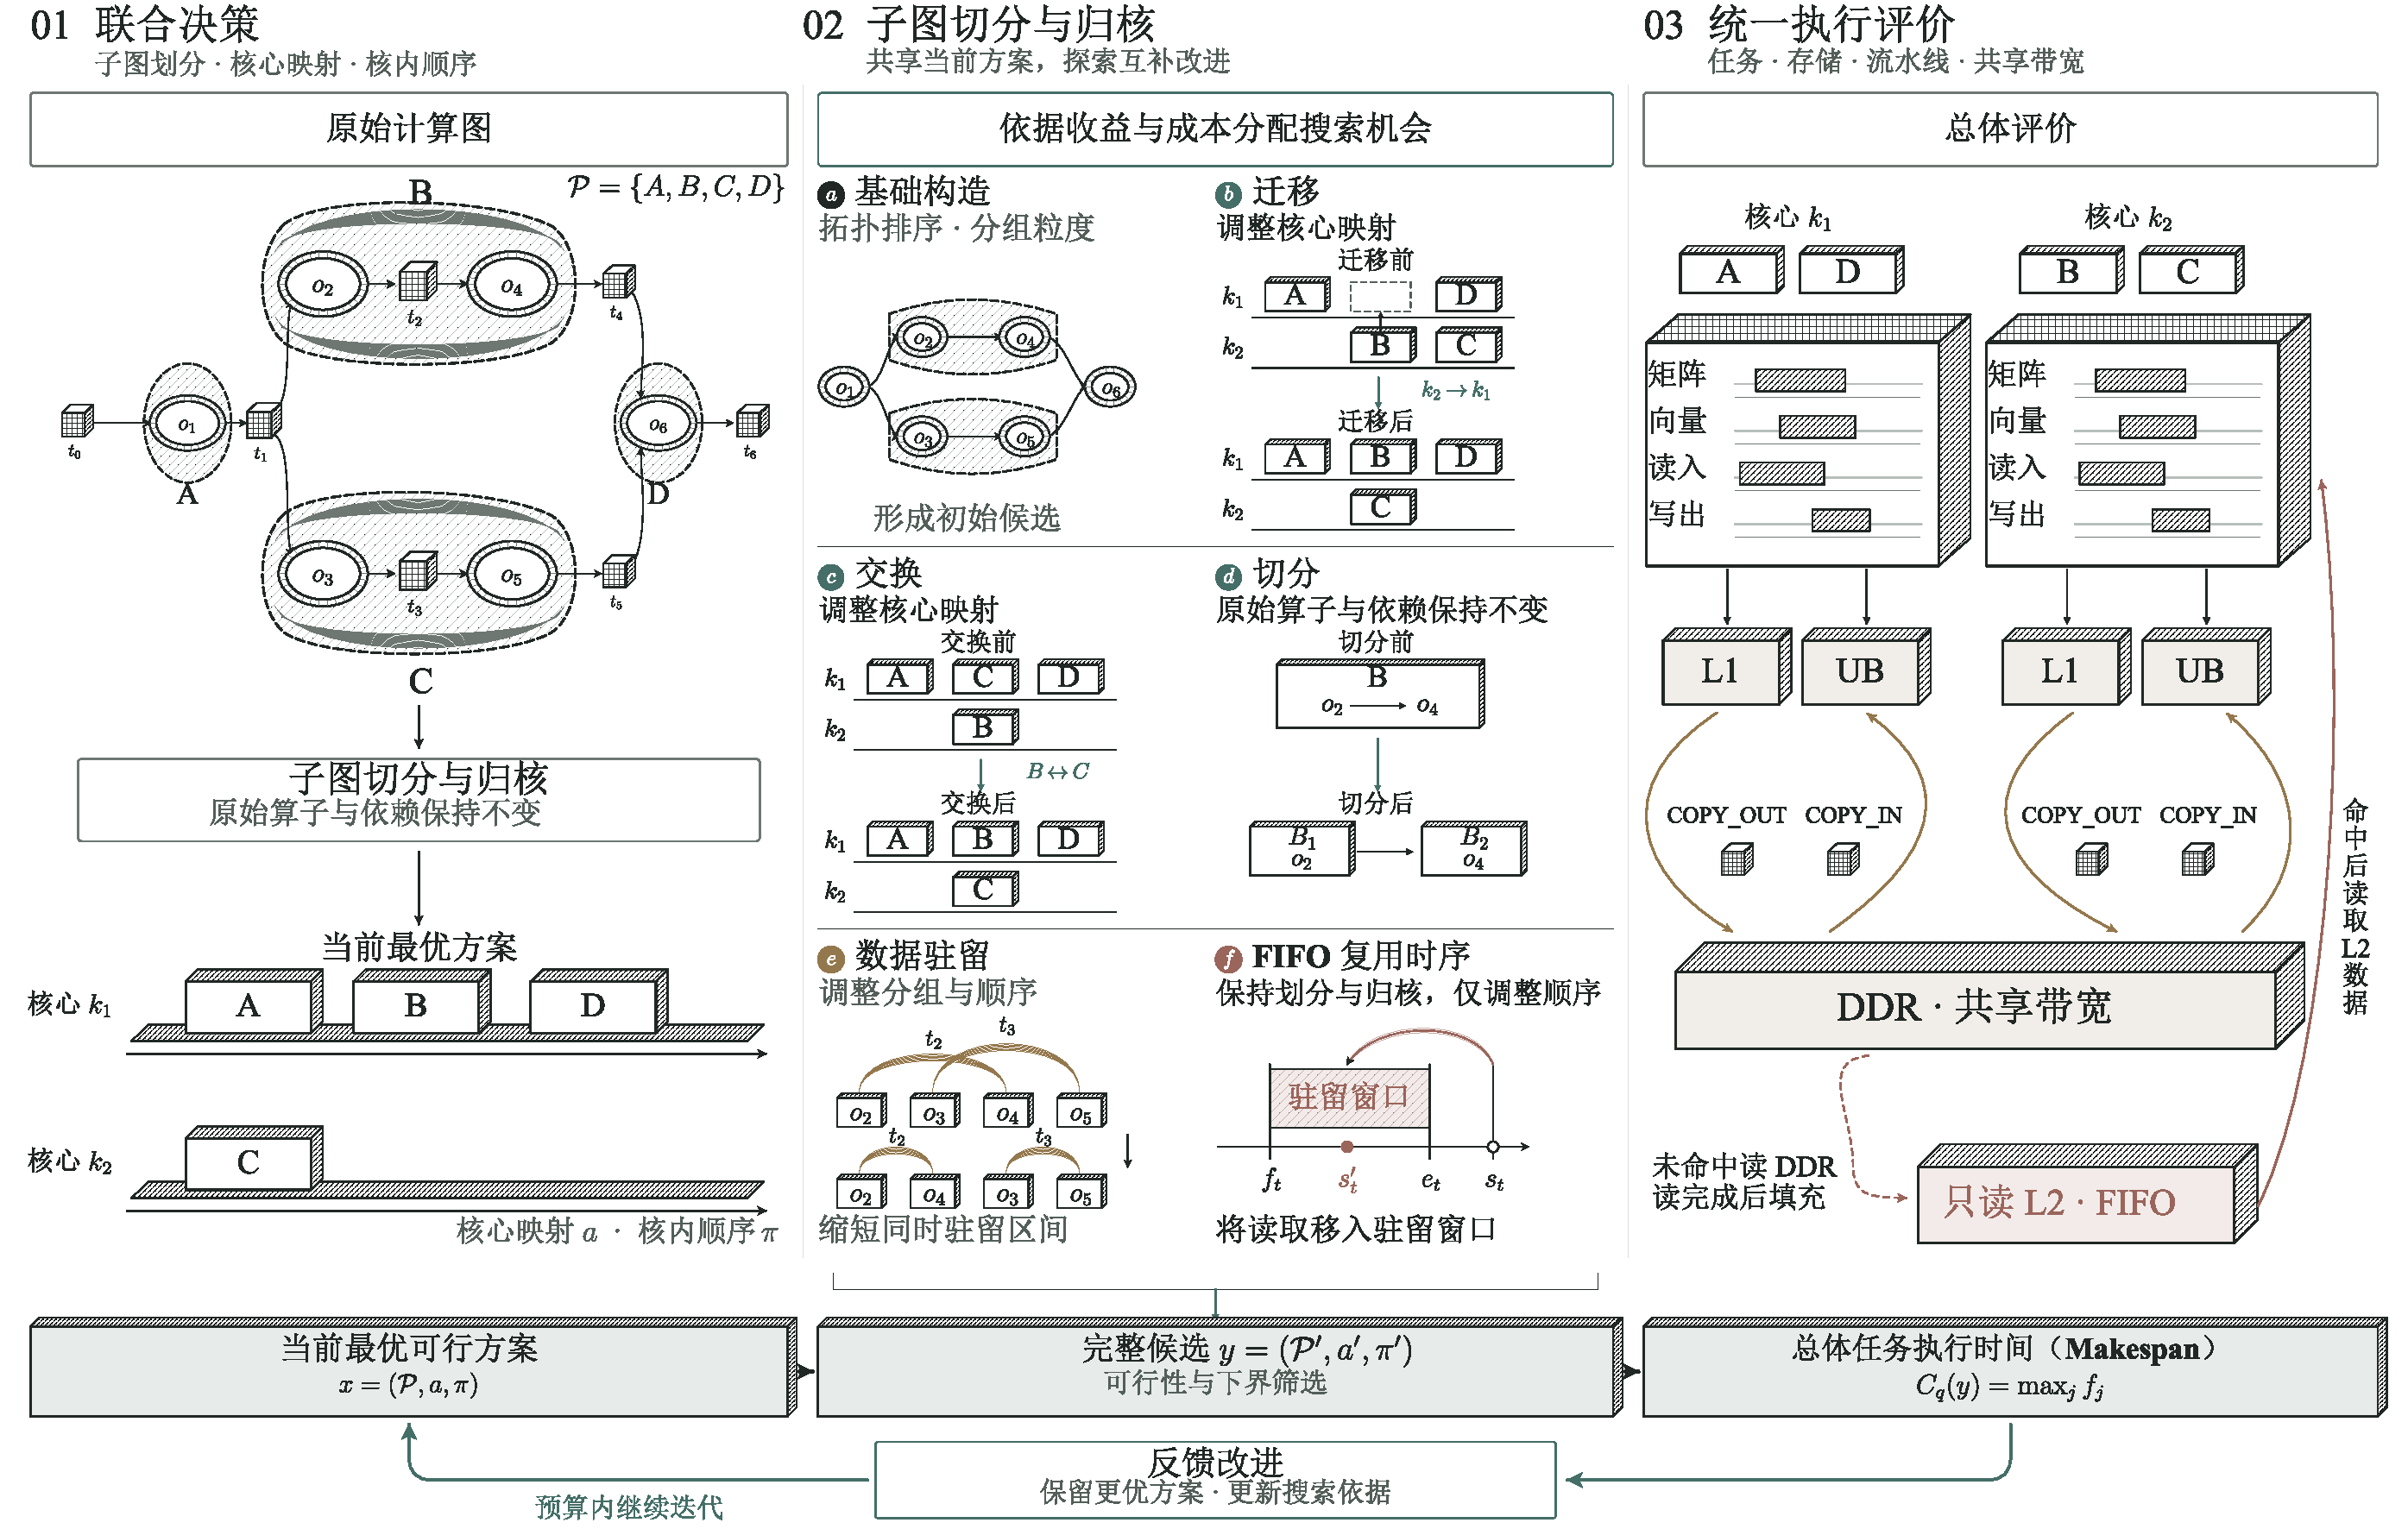
\includegraphics[width=\textwidth]{../../../../paper_a_figures/engraved_workflow/ink_v13/exports/workflow_qinglu_v13.pdf}
\caption{联合决策、候选生成与统一执行评价}\label{fig:roadmap}
\end{figure}

如图~\ref{fig:roadmap} 所示，以子图划分、核心映射和核内顺序组成完整方案，基础构造、迁移、交换、切分、数据驻留与FIFO复用时序调整交替生成候选；问题一使用（a）—（d），问题二增加（e），问题三增加（f），各操作并非串行步骤。候选经可行性与下界筛选后，在任务、存储、流水线及共享带宽约束下统一评价，优先比较总体任务执行时间，相同时比较总额外数据搬运量，保留更优方案，并按收益与成本调整搜索机会。第三问在读入发射时查询只读L2，命中由L2服务，否则由DDR服务，读入完成后按容量和FIFO规则尝试填充。迭代至预算耗尽后输出当前最优可行方案，再固定第三问方案进行无L2与有L2配对评价。
